\chapter{Maximale Flüsse und Matchings}

% helpers
\newcommand{\pluseq}{\mathrel{+}=}
\newcommand{\minuseq}{\mathrel{-}=}

\section{Definitionen}

\subsection{Netzwerk}

Ein \term{Netzwerk}\index{Netzwerk} ist ein gerichteter und gewichteter Graph mit zwei speziellen Knoten --- einer \term{Quelle}\index{Netzwerk!Quelle} und einer \term{Senke}\index{Netzwerk!Senke}.

Unterschied zwischen \( s \), \( t \) und dem Rest der Knoten ist, dass \( s \) keine eingehenden und \( t \) keine ausgehenden Kanten hat. 

Das Gewicht \( c_e \) der Kante \( e \) nennen wir die \term{Kapazität}\index{Netzwerk!Kapazität} der Kante. Diese muss nicht-negativ sein.

\begin{figure}[H]
  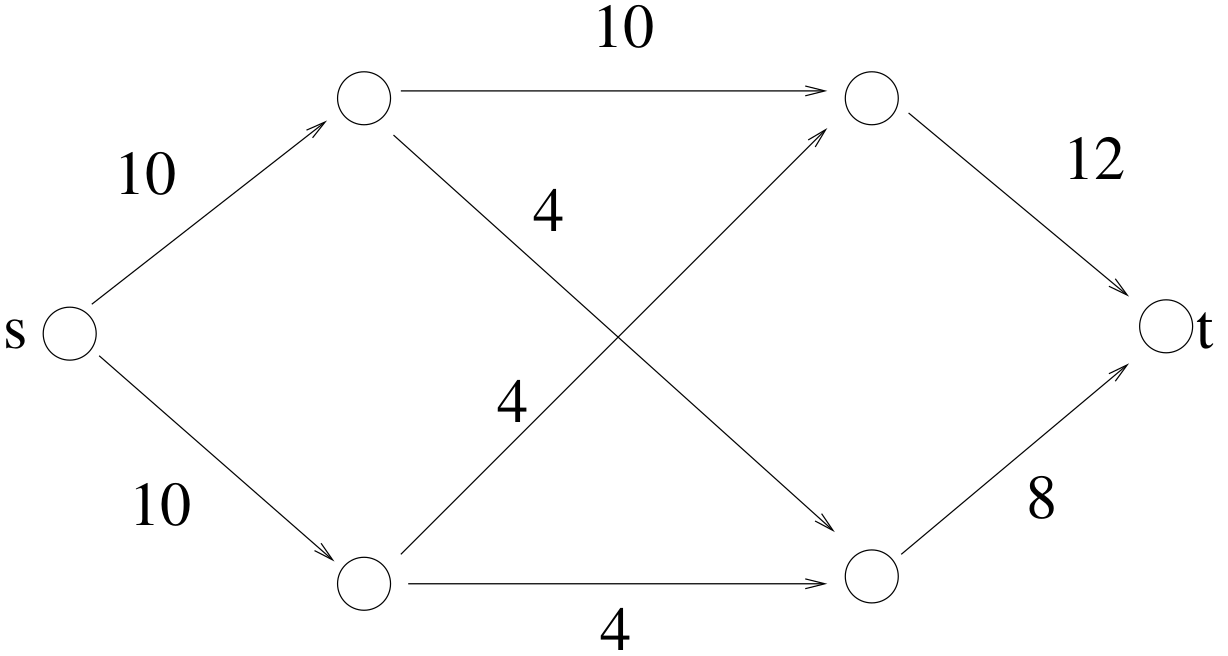
\includegraphics[width=0.6\textwidth]{network}
  \caption{Beispiel für ein Netzwerk mit Quelle \( s \) (\emph{source}) und Senke \( t \) (\emph{sink})}
\end{figure}

\subsection{Fluss}

Ein \term{Fluss}\index{Fluss} in einem Netzwerk ist eine Funktion \( f_e \) auf den Kanten des Netzwerks. Ein Fluss hat folgende Eigenschaften:

\begin{itemize}
  \item \( 0 \leq f_e \leq c_e \) (\( \forall e \in E \))
  \item \( \forall v \in V \setminus \left \{ s,t \right \} : \) Summe eingehender Flüsse = Summe ausgehender Flüsse
\end{itemize}

Wir definieren außerdem den \term{Wert}\index{Fluss!Wert} eines Flusses \( f \) als
\begin{equation*}
  \text{val}(f) = \Sigma \text{ von \( s \) ausgehender Fluss} \equiv \Sigma \text{ zu \( t \) eingehender Fluss}
\end{equation*}

Ziel ist es in der Regel, einen Fluss in einem festgelegten Netzwerk mit \emph{maximalem Wert} zu finden.

\section{Cuts}

\begin{definition}[Cut]
  Ein \( s \)-\( t \)-\term{Cut}\index{Cut} ist eine Partitionierung eines Graphen \( G \) in zwei Mengen \( S \) und \( T \), sodass \( s \in S \) und \( t \in T \).

  Die \term{Kapazität}\index{Cut!Kapazität} eines Cuts ist
  \begin{equation*}
    \sum\left \{ c_{(u,v)} : u \in S \wedge v \in T \right \}\text{,}
  \end{equation*}
  also die Summe der Kapazitäten aller Kanten, die durch den Cut ``durchgeschnitten'' werden.
\end{definition}

\begin{figure}[H]
  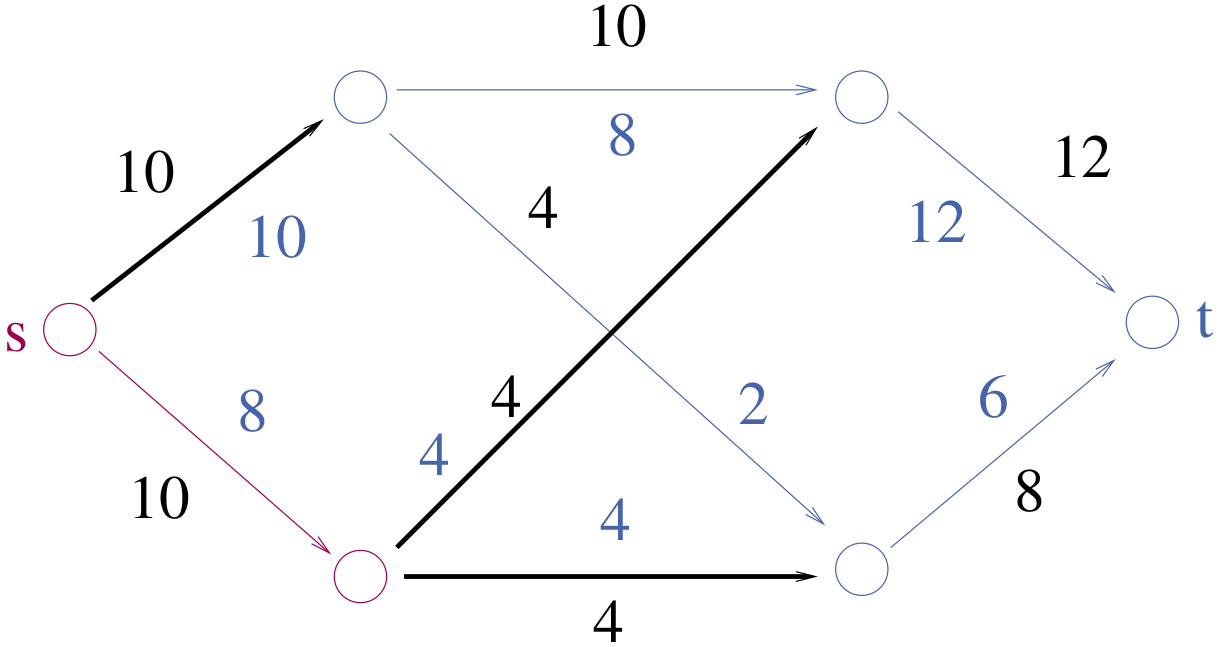
\includegraphics[width=0.6\textwidth]{flow}
  \caption{Die blauen Zahlen stellen einen möglichen Fluss in obigem Netzwerk dar. Die schwarzen Kanten sind ein möglicher Cut. Der Wert dieses Flusses ist 18}
\end{figure}

Es gilt folgender extrem praktischer Satz:

\begin{theorem}[Fluss-Cut-Dualität]
  Der Wert eines maximalen \( s \)-\( t \)-Flusses ist die minimale Kapazität eines \( s \)-\( t \)-Cuts.
\end{theorem}

Wie können wir nun diesen Satz nutzen, um einen maximalen Fluss zu finden? Eine Möglichkeit ist \emph{Lineare Programmierung}, aber es gibt bessere Lösungen.

\section{Pfade augmentieren}

Idee ist folgende:
\begin{enumerate}
  \item Wähle einen \( s \)-\( t \)-Pfad, der noch Kapazität übrig hat.
  \item Sättige die Pfadkante mit der kleinsten Restkapazität.
  \item Korrigiere die Kapazitäten aller anderen Kanten mithilfe des \emph{Residualgraphen} und starte wieder von vorne.
\end{enumerate}

\subsection{Residualgraph}

Ist ein Netzwerk \( G = (V, E, c) \) mit Fluss \( f \) gegeben, so erhalten wir den \term{Residualgraphen}\index{Residualgraph} \( G_f = (V, E_f, c^f) \). Dabei gilt für jedes \( e \in E \):
\begin{equation*}
  \begin{cases}
    e \in E_f \text{ mit } c_e^f = c_e - f(e) \quad &\text{falls } f(e) < c(e)  \\
    e^\text{rev} \in E_f \text{ mit } c_{e^\text{rev}}^f = f(e) \quad &\text{falls } f(e) > 0
  \end{cases}
\end{equation*}
Dabei ist für \( e = (u,v) \in E \) die Kante \( e^\text{rev} = (v,u) \).

Die Kanten in die ``normale'' Richtung sind also diejenigen, die noch Restkapazität haben; die neue Kapazität ist die Restkapazität.

Die Kanten in umgekehrte Richtung sind die Kanten, wo der Fluss \( > 0 \) ist (das heißt insbesondere, dass auch beide Fälle eintreten können). Das Gewicht dieser Kanten entspricht dem Fluss der Kanten in normale Richtung.

\begin{minipage}{.475\textwidth}
  \begin{figure}[H]
    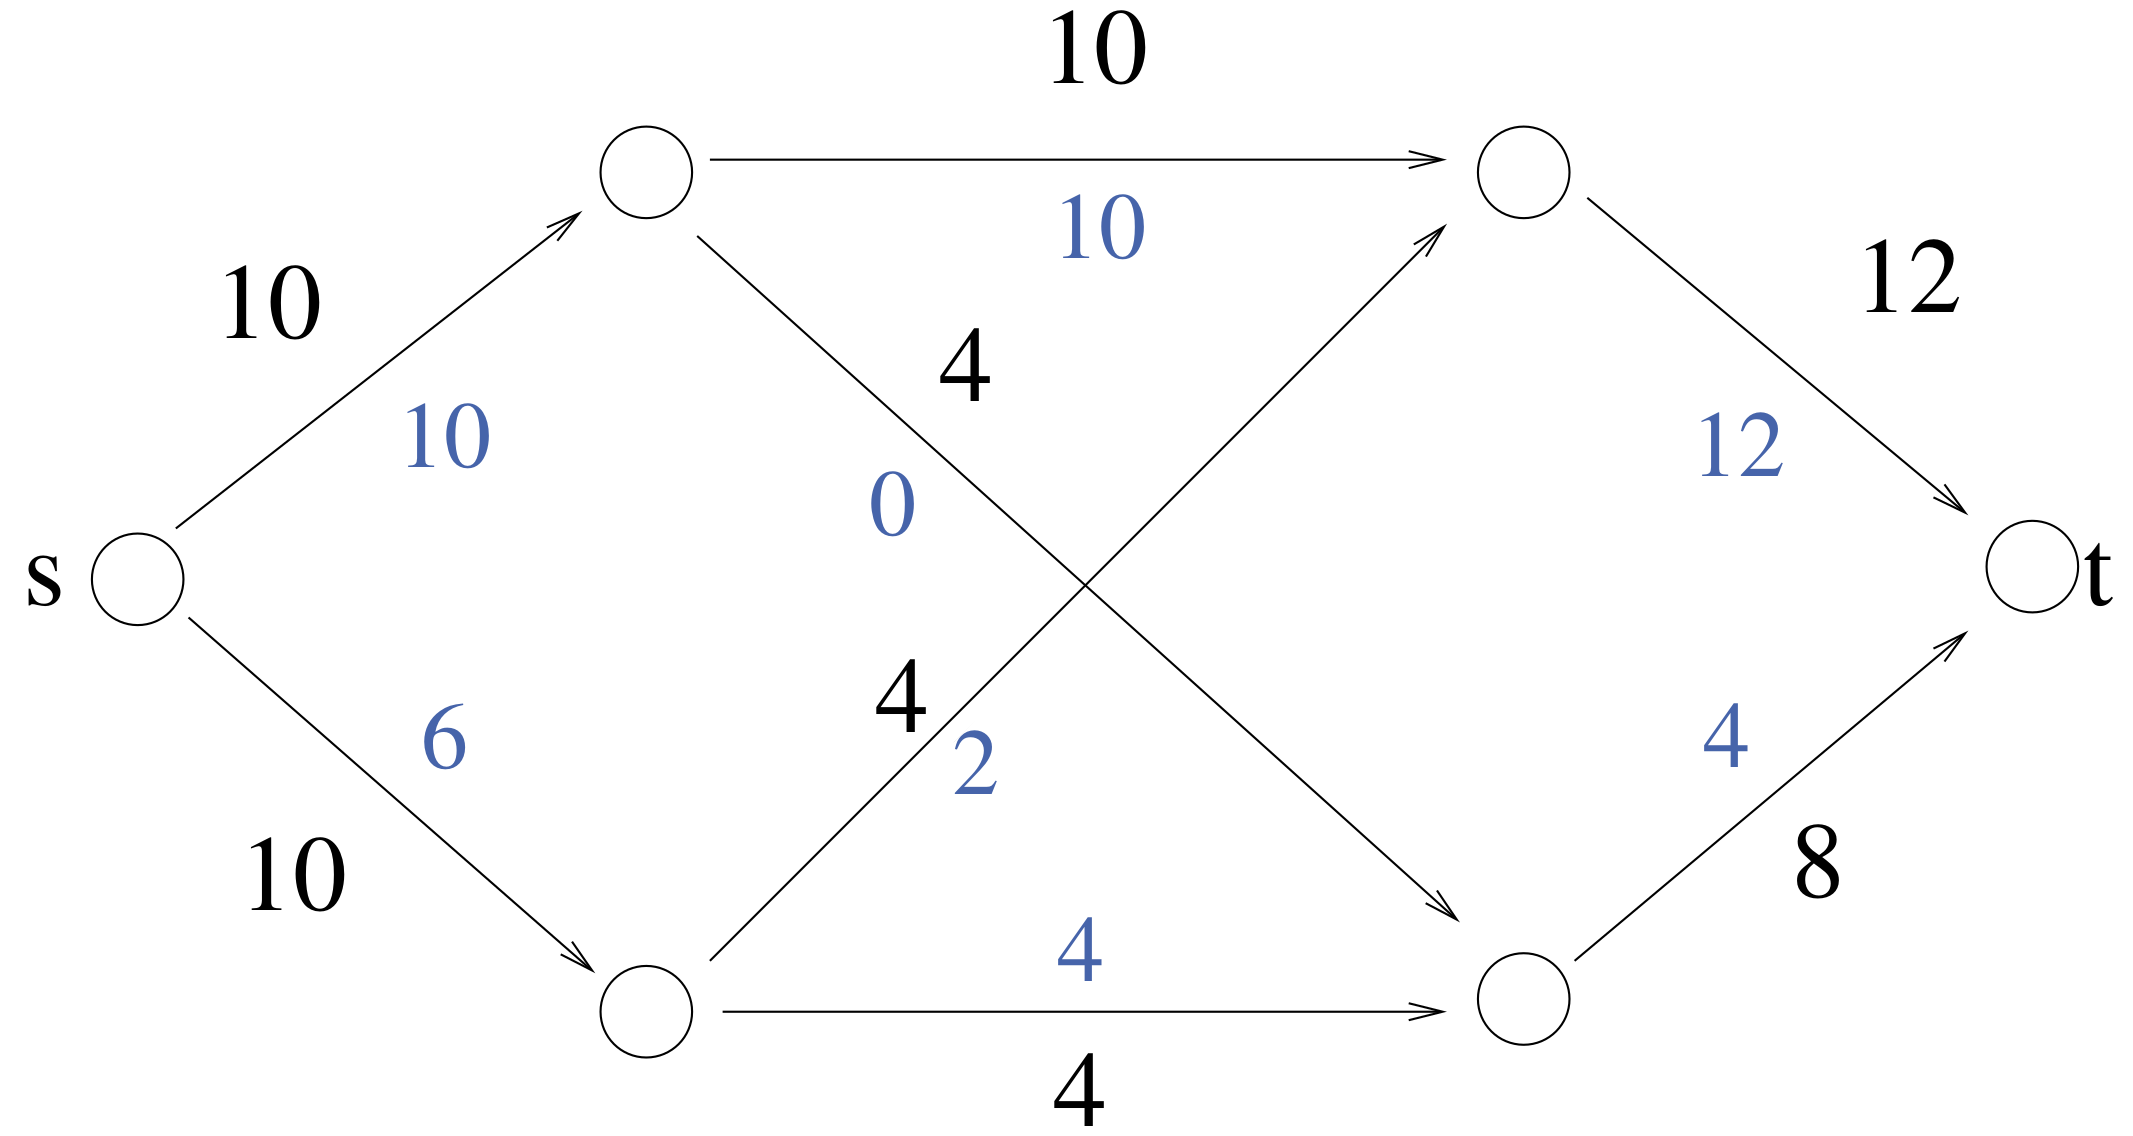
\includegraphics[width=\textwidth]{flow2}
    \caption{Nochmal der Fluss von oben}
  \end{figure}
\end{minipage}
\hfill
\begin{minipage}{.475\textwidth}
  \vspace{6.8mm}
  \begin{figure}[H]
    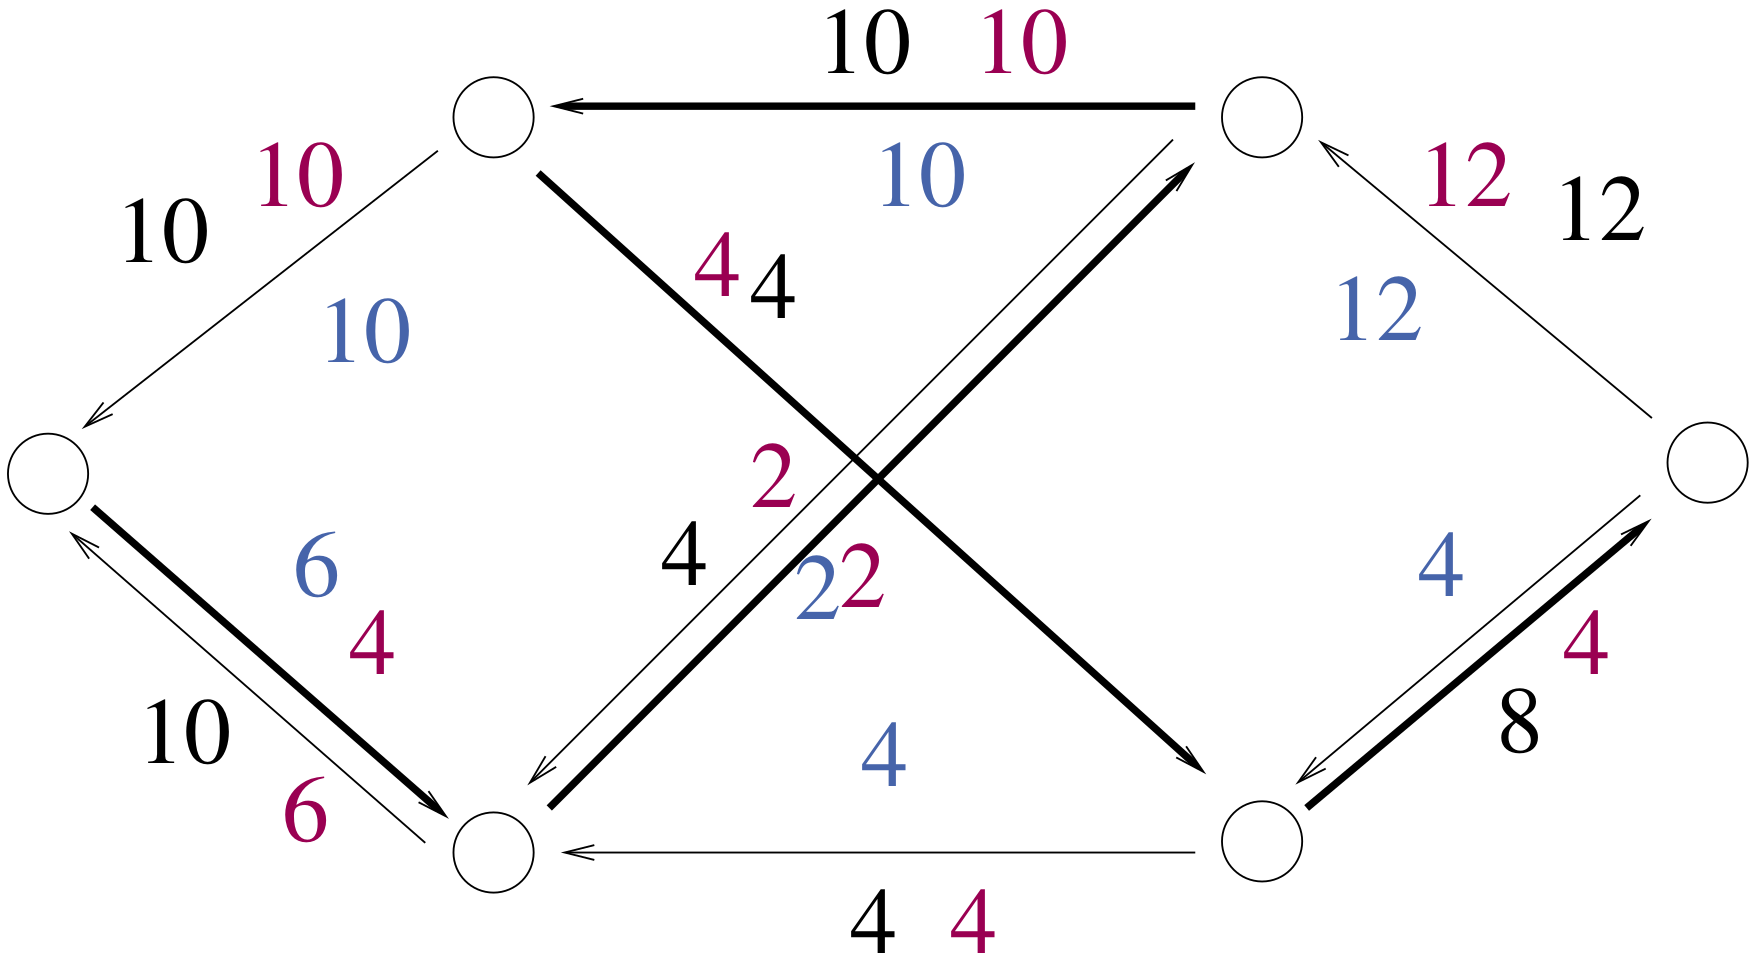
\includegraphics[width=\textwidth]{residualFlow}
    \caption{Der zu nebenstehendem Fluss gehörende Residualgraph. Schwarz die Kapazität, Blau der Fluss, Rot die residuale Kapazität}
  \end{figure}
\end{minipage}

Wir suchen jetzt nach einem \( s \)-\( t \)-Pfad \( p \), sodass jede Kante residuale Kapazität \( c_e^f \neq 0 \) hat:

\begin{pseudocode}
  \( \Delta f \coloneqq \min_{e \in p}c_e^f \) \\
  \textbf{foreach} \( (u,v) \in p \) \textbf{do} \\
  \phantom{\enskip} \textbf{if} \( (u,v) \in E \) \textbf{then} \( f_{(u,v)} \pluseq \Delta f \) \\
  \phantom{\enskip} \textbf{else} \( f{(v,u)} \minuseq \Delta f \)
\end{pseudocode}

Wir können nun den \term{Ford-Fulkerson-Algorithmus}\index{Ford-Fulkerson-Algorithmus} implementieren:

\begin{pseudocode}
  \textbf{\textsc{FFMaxFlow}}\( (G = (V,E), s, t, c: E \to \N) : E \to \N \) \\
  \phantom{\enskip} \( f \coloneqq 0 \) \\
  \phantom{\enskip} \textbf{while} \( \exists \) path \( p = (s,\dots,t) \) in \( G_f \) \textbf{do} \\
  \phantom{\enskip} \phantom{\enskip} augment \( f \) along \( p \) \\
  \phantom{\enskip} \textbf{return} f
\end{pseudocode}

Die Zeitkomplexität ist \( O(m*\text{val}(f)) \), da bei jedem Durchgang der Fluss um mindestens \( 1 \) erhöht wird und jedes Mal DFS \( O(m) \) ausgeführt werden muss.

\subsection{Problem --- Blocking Flows}

\begin{minipage}{.6\textwidth}
  Es gibt Netzwerke, in denen der Ford-Fulkerson-Algorithmus tatsächlich die längstmögliche Laufzeit braucht, obwohl die Lösung sehr trivial ist. Grund dafür sind sogenannte \term{Blocking Flows}\index{Fluss!Blocking Flow}.

  \( f_b \) ist ein \emph{blocking flow} in \( H \), falls für jeden \( s \)-\( t \)-Pfad \( p \) gilt:
  \begin{equation*}
    \exists \ e \in p : f_b(e) = c(e)\text{.}
  \end{equation*}
  Das bedeutet, dass jeder \( s \)-\( t \)-Pfad eine vollständig ausgelastete Kante beinhaltet.
\end{minipage}
\hfill
\begin{minipage}{.35\textwidth}
  \begin{figure}[H]
    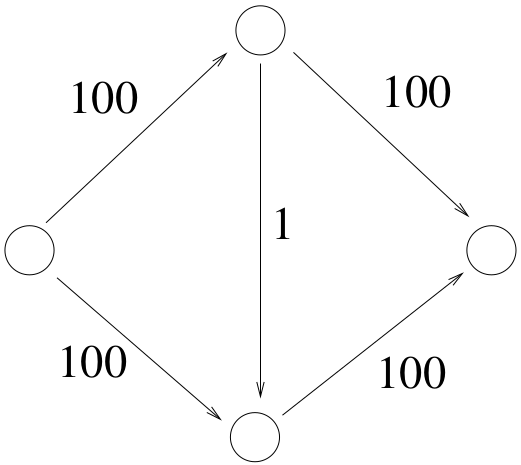
\includegraphics[width=\textwidth]{fulkersonBad}
    \caption{In diesem Netzwerk könnte der Ford-Fulkerson-Algorithmus stets einen Pfad über die mittlere Kante augmentieren und würde deswegen 200 Schritte brauchen}
  \end{figure}
\end{minipage}

\section{Dinic-Algorithmus}

Der \term{Dinic-Algorithmus}\index{Dinic-Algorithmus} sieht so aus:

\begin{pseudocode}
  \textbf{\textsc{DinitzMaxFlow}}\( (G = (V, E), s, t, c: E \to \N) : E \to \N \) \\
  \phantom{\enskip} \( f \coloneqq 0 \) \\
  \phantom{\enskip} \textbf{while} \( \exists \) path \( p = (s,\dots,t) \) in \( G_f \) \textbf{do} \\
  \phantom{\enskip} \phantom{\enskip} \( d = G_f\text{.\textcolor{red}{reverseBFS}}(t) : V \to \N \) \\
  \phantom{\enskip} \phantom{\enskip} \( \textcolor{red}{L_f} \coloneqq (V, \left \{ (u,v) \in E_f : d(v) = d(u) - 1 \right \}) \) \enskip{} \textcolor{gray}{// layer graph} \\
  \phantom{\enskip} \phantom{\enskip} \textcolor{red}{find blocking flow} \( f_b \) in \( L_f \) \\
  \phantom{\enskip} \phantom{\enskip} augment \( f \pluseq f_b \) \\
  \phantom{\enskip} \textbf{return} \( f \)
\end{pseudocode}

Die rot gekennzeichneten Funktionen/Objekte müssen wir noch klären.

Der Ablauf lässt sich folgendermaßen zusammenfassen:

\begin{enumerate}
  \item Berechne Distanz-Labels (Abstand zur Senke) für alle Knoten des Graphen.

   (Rückwärtsgerichtete Breitensuche von \( t \) aus)
  \item Stelle auf Basis der Distanz-Labels den Layer-Graph auf.
  \item Suche auf dem Layer-Graph einen blockierenden Fluss zwischen \( s \) und \( t \).
  \item Führe den gefundenen blockierenden Fluss auf dem Residualgraph aus und aktualisiere diesen entsprechend.
  \item Konstruiere den aktualisierten Layer-Graphen und gehe zu Schritt 3.
  \item Breche ab, sobald kein weiterer Fluss im Layer-Graph existiert.
\end{enumerate}

\subsection{Abstandsfunktion}

Die Abstandsfunktion \( d \) gibt den Abstand eines Knotens zur Senke \( t \) an.

\subsection{Layer-Graph}

Den \term{Layer-Graph}\index{Layer-Graph} eines Netzwerks erhält man, indem man alle Kanten aus dem Residualgraphen entfernt, die nicht von einer Schicht in die vorherige führen. Es werden also alle Kanten
\begin{itemize}
  \item innerhalb einer Schicht und
  \item zwischen Schicht \( i \) und \( i + k \) (\( k \in \N \))
\end{itemize}
entfernt. Formal ist das
\begin{equation*}
  L_f = (V, \left \{ (u,v) \in E_f : d(v) = d(u) - 1 \right \})\text{.}
\end{equation*}

Die Laufzeit des Dinic-Algorithmus ist damit in \( O(mn^2) \).

\section{Matchings}

Ein \term{Matching}\index{Matching} in einem ungerichteten Graphen \( G = (V, E) \) ist eine Teilmenge der Kanten, sodass es keine Kanten gibt, die einen gemeinsamen Knoten berühren.

Ein Matching ist \emph{maximal}, wenn es keine Kante gibt, die man aus \( E \) zum Matching hinzufügen könnte, ohne die Matching-Anforderung zu verletzen.

Ein Matching hat \emph{maximale Kardinalität}, wenn es kein Matching auf \( G \) gibt, dass mehr Knoten abdeckt.

Wir werden Matchings zuerst einmal verwenden, um Flüsse zu berechnen.

\section{Preflow-Push}

Nachteil der pfadaugmentierenden Algorithmen von vorhin ist, dass man Pfade mit hoher Kapazität sehr häufig durchgehen muss aufgrund von späteren Kanten mit geringer Kapazität.

\term{Preflow-Push-Algorithmen}\index{Preflow-Push-Algorithmus} lösen dieses Problem.

\begin{definition}[Preflow]
  Ein \term{Preflow}\index{Preflow} ist ein Fluss \( f \), bei dem die Summe der eingehenden Flüsse für einen Knoten höher sein darf als die Summe der ausgehenden Flüsse. Die Differenz dieser Summen nennen wir den \term{Exzess}\index{Exzess} des Knotens:
  \begin{equation*}
    \text{excess}(v) \coloneqq \underbrace{\sum_{(u,v) \in E} f_{(u,v)}}_{\text{inflow}} - \underbrace{\sum_{(v,w) \in E} f_{(v,w)}}_{\text{outflow}} \geq 0\text{.}
  \end{equation*}
  Wir nennen einen Knoten \( v \in V \setminus \left \{ s, t \right \} \) \term{aktiv}, falls \( \text{excess}(v) > 0 \).
\end{definition}

Wir definieren nun die \code{push}\index{Push}-Funktion:

\begin{pseudocode}
  \textbf{\textsc{push}}\( (e = (v,w), \delta) \) \\
  \phantom{\enskip} \textbf{assert} \( \delta > 0 \) \\
  \phantom{\enskip} \textbf{assert} \(  \text{excess}(v) \geq \delta \) \\
  \phantom{\enskip} \textbf{assert} residual capacity of \( e \geq \delta \) \\
  \phantom{\enskip} \( \text{excess}(v) \minuseq \delta \) \\
  \phantom{\enskip} \( \text{excess}(w) \pluseq \delta \) \\
  \phantom{\enskip} \textbf{if} \( e \) is reverse edge \textbf{then} \( f(\text{reverse}(e)) \minuseq \delta \) \\
  \phantom{\enskip} \textbf{else} \( f(e) \pluseq \delta \)
\end{pseudocode}

Wir nennen einen Push
\begin{itemize}
  \item \term{saturierend}\index{Push!saturierend}, falls \( \delta = c_e^f \),
  \item \term{nicht-saturierend}\index{Push!nicht saturierend}, falls \( \delta < c_e^f \).
\end{itemize}

\subsection{Level-Funktion}

Idee ist nun, von \( s \) aus Richtung \( t \) zu pushen. Dazu benötigen wir eine Approximation \( d(v) \) der BFS-Distanz von \( v \) zu \( t \) in \( G_f \).

Wir können nun den Preflow-Push-Algorithmus implementieren:

\begin{pseudocode}
  \textbf{\textsc{genericPreflowPush}}\( (G = (V, E), f) \) \\
  \phantom{\enskip} \textbf{forall} \( e = (s,v) \in E \) \textbf{do} \( \text{push}(e, c(e)) \) \\
  \phantom{\enskip} \( d(s) \coloneqq n \), \( d(v) = 0 \) for all other nodes \\
  \phantom{\enskip} \textbf{while} \( \exists \ v \in V \setminus \left \{ s, t \right \} : \text{excess}(v) > 0 \) \textbf{do} \\
  \phantom{\enskip} \phantom{\enskip} \textbf{if} \( \exists \ e = (v,w) \in E_f : D(w) < d(v) \) \textbf{then} \enskip \textcolor{gray}{// eligible edge} \\
  \phantom{\enskip} \phantom{\enskip} \phantom{\enskip} choose some \( \delta \leq \min \left \{ \text{excess}(v), c_e^f \right \} \) \\
  \phantom{\enskip} \phantom{\enskip} \phantom{\enskip} \( \text{push}(e,\delta) \) \enskip \textcolor{gray}{// no new steep edges} \\
  \phantom{\enskip} \phantom{\enskip} \textbf{else} \( d(v) \)++ \enskip \textcolor{gray}{// relabel; no new steep edges}
  \phantom{\enskip}
\end{pseudocode}

Dieser generische Algorithmus hat eine Laufzeit von \( O(n^2m) \). 

\subsection{Highest Level Preflow Push}

Wählt man immer die aktiven Knoten aus, die \( d(v) \) maximieren, so kann man die Laufzeit auf \( O(n^2\sqrt{m}) \) drücken.

Mit heuristischen Mitteln wie agressivem lokalen Relabeling lässt sich der practical case weiter reduzieren.